Today, we will continue our exploration of zero-dimensional path integrals in quantum field theory.
\subsection*{Interacting theory}
Let us consider a single real scalar field $\phi:\set{\text{point}}\to \RR$. We choose the action
\begin{equation}
    S(\phi)=\frac{1}{2} m^2 \phi^2 +\frac{\lambda}{4!} \phi^4.
\end{equation}
We'll take $\lambda >0$ for stability%
    \footnote{That is, we cannot make $S$ arbitrarily negative by going to large values of $\phi$. This is equivalent to requiring that our theory has a true vacuum at $\phi=0$.}
and $m^2>0$ such that $\min(S)$ lies at $\phi=0$ so that we can easily expand around the minimum of $S$.

The path integral is then
\begin{equation}
    Z = \int d\phi \exp \bkt{
        -\frac{1}{\hbar}\paren{\frac{1}{2} m^2 \phi^2 +\frac{\lambda}{4!}\phi^4}
    }.
\end{equation}
This will be equivalent to expanding about $\hbar = 0$ (semi-classical limit).
We can obviously open up the exponential and rewrite as a series in $\phi$ and $\hbar,$
\begin{align*}
    Z &= \int d\phi e^{-\frac{m^2 \phi^2}{2\hbar}} \sum_{n=0}^\infty \frac{1}{n!} \paren{-\frac{\lambda}{\hbar \,4!}
    }^n \phi^{4n}\\
    &=\frac{\sqrt{2\hbar}}{m} \sum_{n=0}^\infty \frac{1}{n!} \paren{ -\frac{\hbar \lambda}{4! m^4}
    }^n \cdot
    2^{2n} \int_0^\infty dx e^{-x} x^{2n+\frac{1}{2} -1},
\end{align*}
where we have performed a change of variables $x=\frac{m^2 \phi^2}{2\hbar}$. The integral in this expression is in fact just a gamma function,%
    \footnote{The gamma function is defined by $\Gamma(z)=\int_0^\infty dx\, x^{z-1} e^{-x}.$}
%
\begin{equation*}
    \Gamma\paren{2n+\frac{1}{2}}=\frac{(4n)! \sqrt{\pi}}{4^{2n}(2n)!}.
\end{equation*}
Thus our path integral computation using the gamma function is
\begin{equation}\label{zerodpathintegralphi4}
    Z=\frac{\sqrt{2\pi \hbar}}{m} \sum_{n=0}^N \paren{-\frac{\lambda \hbar}{m^4}
    }^n \underbrace{\frac{1}{(4!)^n n!}}_{(1)} \underbrace{\frac{(4n)!}{2^{2n}(2n)!}}_{(2)}.
\end{equation}
Note that from Stirling's approximation, $n!\approx e^{n\log n}$, Thus these two combinatorial-looking terms scale roughly as $e^{n\log n}\approx n!$. The factorial growth of the coefficients means that this path integral actually has zero radius of convergence. This is an asymptotic series-- it looks like it is getting better and better, and then everything goes to hell.%
    \footnote{What we mean by an asymptotic series is that it converges not in the limit as the number of terms in the power series gets very large but rather as the expansion parameter gets very small.}

In practice the ``true'' function can differ from the truncated series by some transcendental function which might be small. Cf. Skinner Ch. 2 for more discussion of asymptotic series.

Note that term (1) in the path integral series expansion \ref{zerodpathintegralphi4} comes from expanding the $\frac{\lambda}{4! \hbar} \phi^4$ term in the exponent, while term (2) is the number of ways of joining $4n$ elements in distinct pairs (compare our discussion at the end of the previous lecture). We can associate some Feynman diagrams to this-- a propagator and a four-point vertex.
\begin{center}
    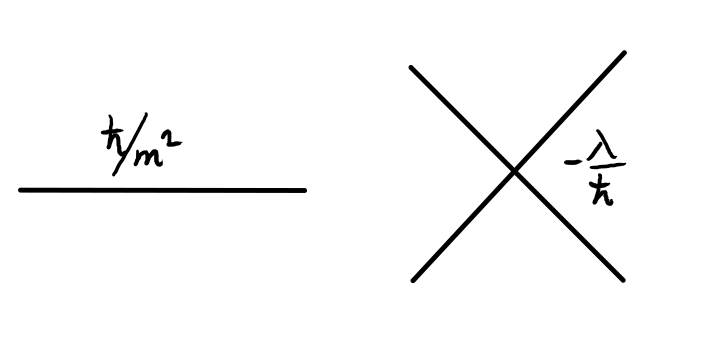
\includegraphics[width=0.5\textwidth]{2019/01/20190124_fourpointfeynman.png}
\end{center}

Note also that $Z$ has no $\phi$ dependence, meaning that the Feynman diagrams have no external legs. Let $D_n$ be the set of \emph{labelled} vacuum diagrams with $n$ vertices, so that $D_1$ is the following set of diagrams, with $|D_1|=3$.

\begin{center}
    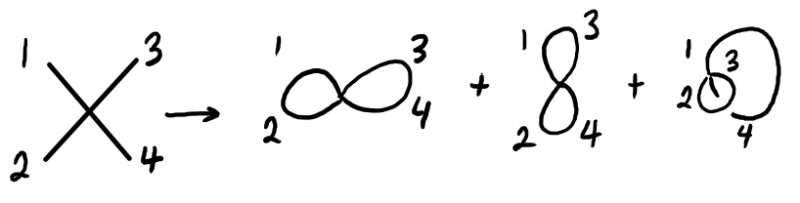
\includegraphics[width=0.75\textwidth]{2019/01/20190124_labeledfourpoint.png}
\end{center}

Then let $G_n$ be the group which permutes each of the 4 fields at each vertex ($(S_4)^n$) and also permutes the $n$ vertices ($S_n$). The size of this group is
\begin{equation*}
    |G_n|=|S_4|^n |S_n| = (4!)^n n!.
\end{equation*}
We therefore recognize that
\begin{align*}
    \frac{Z}{Z_0} &= \sum_{n=0}^N \paren{
        -\frac{\lambda \hbar}{m^4}
    }^n \frac{|D_n|}{|G_n|}\\
    &= 1-\frac{\hbar \lambda}{8m^4} + \frac{35}{384} \frac{\hbar^2\lambda^2}{m^8} + \ldots
\end{align*}
with $Z_0=\frac{\sqrt{2\pi\hbar}}{m}$. Physically, we can consider $\frac{|D_n|}{|G_n|}$ to be the sum over topologically distinct graphs divided by a symmetry factor. Equivalently, we write
\begin{equation}
    \frac{|D_n|}{|G_n|}=\sum_\Gamma \frac{1}{S_\Gamma}
\end{equation}
where $\Gamma$ is a distinct graph free from labels and $S_\Gamma$ is the number of permutations of lines and vertices leaving $\Gamma$ invariant. Some examples appear in Fig. %figure ref here

In dimensions $>0$, loops correspond to integrals over internal momenta, so these diagrams may have different contributions aside from the symmetry factors.

If we introduce an external source, then our path integral has a generating function
\begin{equation}
    Z(J)=\int d\phi \exp -\frac{1}{\hbar}\paren{
    \frac{1}{2}m^2 \phi^2 +\frac{\lambda}{4!}\phi^4 +J\phi
    }
\end{equation}
and our correlation functions are modified as before, with $\avg{\phi^2}=\frac{(-\hbar)^2}{Z(0)}\left.\frac{\p^2}{\p J^2} Z(J)\right|_{J=0}$. Source terms correspond to lines terminating on vertices $J$, so that the expansion of $Z(J)$ involves not only $Z(0)$ vacuum diagrams but also diagrams that terminate with even numbers of source vertices.